\newcommand{\rect}[2]{%
    \fill[pink] (#1-1,0,#2-1) rectangle (#1,0,#2);
}

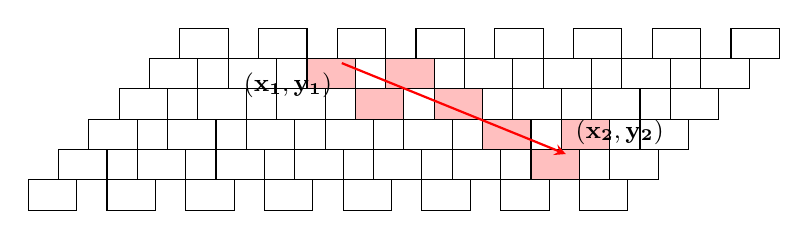
\begin{tikzpicture}[font=\sffamily]
    \rect{3}{2}
    \rect{4}{2}
    \rect{4}{3}
    \rect{5}{3}
    \rect{6}{4}
    \rect{7}{4}
    \rect{7}{5}
    % Draw 8×6 grid
    \foreach \x in {0,...,7} {
        \foreach \y in {0,...,5} {
            \draw[black] (\x,0,\y) rectangle (\x+1,0,\y+1);
        }
    }
    \draw[thick, -stealth, red] (2.5,0,1.15) -- (6.5,0,4.15);
    \node at (2.5,0,1.15) [below left] {\small $\mathbf{(x_1, y_1)}$};
    \node at (6.5,0,4.15) [above right] {\small $\mathbf{(x_2, y_2)}$};
\end{tikzpicture}